\section{Network analysis}
Una rete è un insieme di entità con proprietà simili chiamate nodi, connesse da archi. Questi possono essere reali, dinamici, astratti, \dots, ma ogni tipologia può essere rappresentata da un grafo. 

Terminologia:
\begin{itemize}
	\item Arco diretto (indiretto), ha una direzione (nodo di entrata e di uscita);
	\item Attributo, caratteristica associata a un arco come il peso, il ranking, la tipologia;
	\item Multiarco, più archi collegano la stessa coppia di nodi;
	\item Grafo connesso, esiste un cammino per ogni coppia di nodi.
\end{itemize}

\begin{figure}[h]
	\centering
	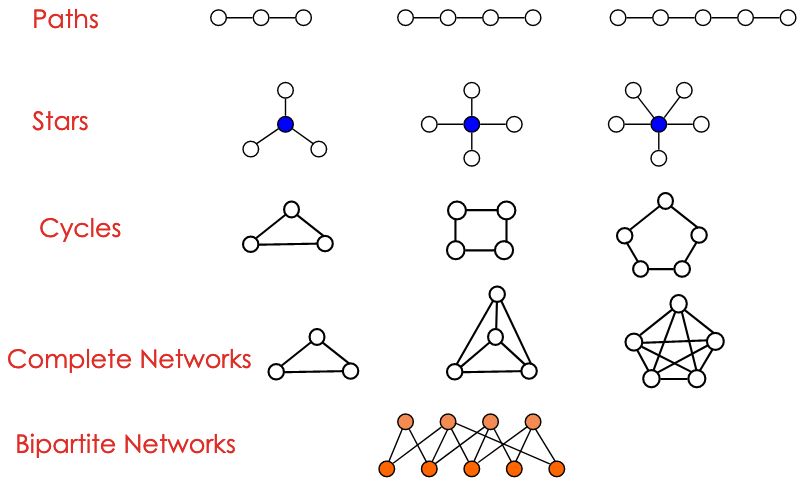
\includegraphics[scale=0.52]{Lezioni/Immagini/network}
\end{figure}

Capire la struttura della rete è importante per le operazioni di gestione e le analitiche. La rappresentazione è generalmente tramite matrice di adiacenza: $A_{ij}$ è 1 se il nodo $i$ ha un arco che lo collega al nodo $j$, 0 altrimenti. Un 1 sulla diagonale indica un ciclo.

Un altro modo per rappresentare un grafo è la lista di adiacenza, più veloce se i nodi sono sparsi e per visualizzare i vicini di ciascuno.

Le reti considerate dalle network analytics sono larghe in termini di nodi, hanno collegamenti sparsi e si evolvono dinamicamente. 

\subsection{Proprietà delle reti}
Le reti complesse sono difficili da visualizzare, quindi si ricorre a misure e statistiche descrittive. Queste servono per indicare la distribuzione dei nodi, il raggruppamento o la centralità.

Il primo concetto da considerare è il grado di un nodo, cioè il numero di archi entranti o uscenti. Formalmente, outdegree$(i) = \sum_{j=1}^{n} A_{ij}$, indegree$(j) = \sum_{i=1}^{n} A_{ij}$ (matrice di adiacenza).

Queste quantità permettono di calcolare il grado totale di un nodo (somma), la media e la distribuzione. $P(k)$ è la probabilità che un nodo casuale abbia grado $k$ (robustezza della rete, diffusione di informazioni). Essa viene calcolata dividendo il numero di nodi con grado $k$ per il totale, e poi normalizzando il valore.

Il numero massimo di archi in una rete di $N$ nodi è:
$$E_{max} = \binom{N}{2} = \frac{N(N - 1)}{2}$$
Un grafo con grado massimo è completo, e il suo grado medio è $N - 1$.

La distribuzione è essenziale per capire il livello di connessione del grafo: se è bassa, la maggior parte dei nodi hanno pochi link, e qualche nodo ne ha molti. I nodi che hanno molti collegamenti in una rete sparsa si definiscono \textbf{hub}, ed è importante capire le motivazioni per cui essi hanno così tanti archi entranti o uscenti.

Legge di \textbf{Metcalfe}: il valore della rete è proporzionale al quadrato del numero dei nodi: più nodi ci sono, più una rete diventa importante (es. fax). Il problema nella realtà è che la maggior parte dei grafi sono sparsi, e gli archi hanno peso differente.

Un cammino è una sequenza di nodi in cui ognuno è adiacente all'altro (connesso da un link), di cui la lunghezza è costituita dal numero di archi. Bisogna tenere conto anche dell'eventuale direzione dei collegamenti, nei grafi diretti. Si hanno:
\begin{itemize}
	\item Distanza, numero di archi appartenenti al cammino più corto tra due nodi;
	\item $N_{ij}$ numero dei cammini più corti estratti dalla matrice di adiacenza;
	\item Visita BFS per trovare i cammini minimi;
	\item Diametro, massima distanza tra una coppia di nodi;
	\item Distanza media, per un grafo diretto, la media delle distanze per ogni coppia.
\end{itemize}

La connessione delle componenti di un grafo può essere determinata osservando la matrice di adiacenza: le parti connesse sono confinate in sottomatrici quadrate.

Il coefficiente di clustering, compreso tra 0 e 1, è la probabilità che due vicini di un nodo abbiano un collegamento. $C_j = 1$ se il grafo è completo. 

Più la rete è densa, quindi, maggiore è il coefficiente: ci si trova in contesti con elevato numero di archi. La media può dare un'idea generale del grado di clustering.


